\chapter{Introduction}
In this chapter, the reader is introduced to the dementia disease, the current methods for its detection, the consequences and what scientists think might be the cause of the disease. 

\section{Dementia}

Dementia is not a specific disease but an overall term used to group all diseases that are characterised by a decrease in memory, thinking capabilities, language and other skills related to the thought. With between 60 and 80 percents of the cases, Alzheimer is the most common disease-causing dementia. Despite the fact that dementia is affecting mostly old people, it is not a normal stage of life and therefore should not be seen as severe ageing. 

\begin{figure}
 \centering
 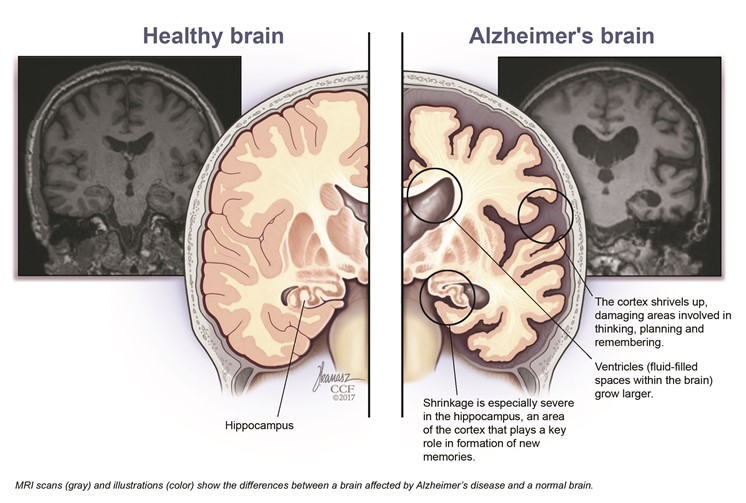
\includegraphics[width=400]{figures/Alzheimer_brain.jpg}
 \caption[Test]{Illustration\footnotemark of the differences between a healthy brain and the brain of someone with Alzheimer disease.}
 \label{fig:alzheimerbrain}
\end{figure}
\footnotetext{\href{https://www.keepmemoryalive.org/brain-science/alzheimers-brain}{https://www.keepmemoryalive.org/brain-science/alzheimers-brain}}

Figure \ref{fig:alzheimerbrain} highlights the visual differences that practitioners can use to distinguish a Alzheimer patient from a control one. Knowing which part of the brain is affected by the disease will help us evaluate our model. We expect a good model to focus his attention on those zone in order to make its prediction. In fact, one would more easily trust a model that has the same attention as a human.

\section{Current Methods}
Most of the current models for detecting dementia are based on comparing some healthy brains with the one from the patient. This requires all the brain scans to be aligned, such that a voxel at a specific coordinate is mapping to the same brain region on both images. Section \ref{sec:coregistration} describes in details how to align two images.

TODO: ADD ANALYSIS


\section{Age vs. Dementia}

It is tempting to see dementia damaged brain as an over aged one. In both cases, we observe a loss of white matter due to neuron death. Even though scientists currently do not know exactly what causes the disease, they do observe the presence of bio-marker such as plaque and tangle \cite{alzheimer_past_present_future}.

Despite the differences, people have built simple dementia detectors by training an age predictor on healthy brains. It appears that their predictor performs badly on dementia's brains and tend to over age people with the disease. As we trained an age predictor on healthy brains, in annexe \ref{chap:age_pred} we took the opportunity to try it on our data. In fact, as shown in the annexe, it turns out that on our data, such a predictor would perform badly. This tends to show that indeed the assumption is wrong and that dement person does not have over-agedd brain.

In general, it would be more interesting to build a model that is able to detect dementia regardless the patient's age, therefore being as little biased as possible with respect to age.